\chapter{地下探测FDTD仿真技术研究}
\section{天线模型仿真}
\subsection{FDTD天线模型原理}
\subsection{仿真实例}
\section{拟真土壤模型}
\subsection{拟真土壤模型原理}
Peplinski 等人提出一种模拟真实土壤电磁特性的半经验模型。在此模型中,土壤由三种成分构成,分别是:
颗粒直径在0.05mm到2.0mm之间的沙土,颗粒直径在0.002mm到0.05mm之间的粉土,以及颗粒直径在0.002
以下的粘土。这三种成分的配比不同可表示不同的土壤类型,进而也影响到其电磁特性。同时,土壤中含水量也对
其电磁特性起重大影响。综合这些因素,土壤的复介电常数$\epsilon_m$由式\ref{eqn:peplinskiall}给出。
\begin{equation} 
	\label{eqn:peplinskiall} 
	\begin{aligned} \epsilon_{m} &=\epsilon_{m}^{\prime}-j \epsilon_{m}^{\prime \prime} \\ 
\epsilon_{m}^{\prime} &=1.15 \left[1+\frac{\rho_{b}}{\rho_{s}}\left(\epsilon_{s}^{\alpha}\right)+m_{v}^{\beta^{\prime}} \epsilon_{f w}^{\alpha}-m_{v}\right]^{1 / \alpha} - 0.68\\ 
\epsilon_{m}^{\prime \prime} &=\left[m_{v}^{\beta^{\prime \prime}} \epsilon_{f w}^{\prime \prime \alpha}\right]^{1 / \alpha} \end{aligned}
\end{equation}

上式中,$\epsilon_{m}^{\prime}$ 与 $\epsilon_{m}^{\prime}$分别是复介电常数
$\epsilon_m$的实部与虚部;$\rho_{b}$ 与 $\rho_{s}$分别是土壤的总密度和其中沙土成分
的密度(单位:$g/cm^3$);$\beta^\prime$与$\beta^{\prime \prime}$分别是与土壤构成
相关的常数,其表达式为\ref{eqn:soil_beta},其中$S$与$C$分别是沙土与粘土的构成比例
($0<S<1, 0<C<1$)。
\begin{equation} 
	\label{eqn:soil_beta}
	\begin{aligned}
\beta^{\prime}&=1.2748-0.519 S-0.152 C \\
\beta^{\prime \prime}&=1.33797-0.603 S-0.166 C
	\end{aligned}
\end{equation}

式\ref{eqn:peplinskiall}中$\epsilon_{f w}^{\prime}$与$\epsilon_{f w}^{\prime \prime}$
分别是土壤中自由水的实部与虚部,其表达式由式\ref{eqn:soil_water}给出。
\begin{equation} 
	\label{eqn:soil_water}
	\begin{aligned}
		\epsilon_{f w}^{\prime}&=\epsilon_{w \infty}+\frac{\epsilon_{w 0}-\epsilon_{w \infty}}{1+\left(2 \pi f \tau_{w}\right)^{2}} \\
		\epsilon_{f w}^{\prime \prime}&=\frac{2 \pi f \tau_{w}\left(\epsilon_{w 0}-\epsilon_{w \infty}\right)}{1+\left(2 \pi f \tau_{w}\right)^{2}}+\frac{\sigma_{\mathrm{eff}}}{2 \pi \epsilon_{0} f} \frac{\left(\rho_{s}-\rho_{b}\right)}{\rho_{s} m_{v}}
	\end{aligned}
\end{equation}
其中,$\epsilon_{w \infty}$是$\epsilon_{f w}^{\prime}$在高频时的极限;$\tau_{w}$为自由水的
弛豫时间常数;$\epsilon_{w 0}$为水的静态相对介电常数,其值为80.1;$\sigma_{\mathrm{eff}}$为有效电导率
,由经验公式\ref{eqn:soil_eff}给出。
\begin{equation}
	\label{eqn:soil_eff}
\sigma_{\mathrm{eff}}=0.0467+0.2204 \rho_{b}-0.4111 S+0.6614 C
\end{equation}

以上便是拟真土壤模型的基本原理,下面讨论如何将此模型应用到探地雷达FDTD仿真中。
按照式\ref{eqn:peplinskiall},在给定土壤构成比例$S$与$C$后,该土壤类型的电磁参量主要由含水量决定。
实际土壤中含水量的分布不是均匀的,因此可定义含水量的最小值与最大值分别为$m_{vmin}$与$m_{vmax}$。
将此含水量范围等距离取$n$个点并代入式\ref{eqn:peplinskiall}便可得到一系列复介电常数
$\epsilon_i(i=1,2,3...n)$ 

得到组成土壤的介质列表之后,接下来了的问题便是考虑这些介质应该如何分布在FDTD三维网格中。文献(https://www.cambridge.org/core/books/fractals-and-chaos-in-geology-and-geophysics/FA8339855DBBF054CCF18D8E5DDFFAC9)
指出地下空间内孔隙度含水量等特性的分布并不是完全随机的而是呈随机分形特征。因此可以利用分形生成算法安排前面得到的一系列介质在FDTD网格
中的分布从而达到对真实土壤较好的模拟效果。

分形在数学中是一种抽象的物体,用于描述自然界中存在的事物。人工分形通常在放大后能展现出相似的形状。 
分形也被称为扩展对称或展开对称。如果在每次放大后,
形状的重复是完全相同的,这被称为自相似。分形在不同的缩放级别上可以是近似相似的。 
分形也包有图像的细节重复自身的意味。一种效率较高的分形数据生成算法是以离散傅里叶变换为基础的。
其算法理论基础是具有分形特征的数据的离散傅里叶变换(DFT)上各频率
的系数$m_f$与频率$f$近似呈幂律关系,即:
\begin{equation}
m_f = \frac{C}{f^{\frac{-(2 D-7)}{2}}}
\end{equation}
其中$D$为分形维度,其值在1到3之间。

因此,可以用以下步骤生成生成复介电常数列表在土壤所在三维空间内FDTD网格的分形分布:

1. 对于尺寸为$x,y,z$的FDTD网格区域,生成相同大小的随机三维数据$\mathbf{A}$。

2. 对$\mathbf{A}$应用三维快速傅里叶变换算法,并将结果进行平移,使零频率处于三维向量
的中心。

3. 设$\mathbf{A}$的中心点的坐标为$(i_c,j_c,k_c)$,对于每一个数据点$\mathbf{A}(i,j,k)$
,计算其与中心点的模,即$L=\sqrt{(i - i_c)^2 + (j - j_c)^2 + (k - j_c)^2}$。

4. 应用公式 $\mathbf{A}(i,j,k) = \mathbf{A}(i,j,k) \frac{1}{L^{\frac{-(2 D-7)}{2}}}$。

5. 对$\mathbf{A}$进行逆傅里叶变换,并将结果归一化并量化为$1$到$n$的整数(对应土壤介质的个数),并在对应位置为FDTD网格的赋予相应
的介质参数。

要获得高度拟真的土壤模型,除了要考虑介质参数分布方面的特征,还要考虑到地形的特征。和土壤介质的分布一样,土壤表面起伏的
形态也符合分形的特征(图\ref{soil_profile})。
\begin{figure}[htbp]
	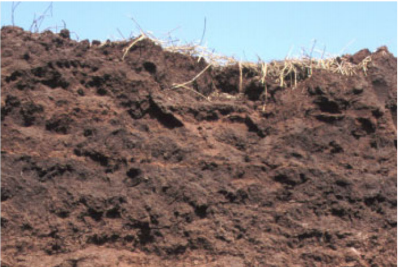
\includegraphics[width=0.8\textwidth]{soil_profile.png}
	\caption{某地土壤切面图,来源 https://www.nrcs.usda.gov}
	\label{soil_profile}
\end{figure}
\subsection{建模实例}
\begin{equation} 
\overline{\varepsilon}=\overline{\mu}=\left[ \begin{array}{ccc}{1+\frac{\sigma_{z}}{j \omega \varepsilon_{0}}} & {0} & {0} \\ {0} & {1+\frac{\sigma_{z}}{j \omega \varepsilon_{0}}} & {0} \\ {0} & {0} & {\frac{1}{1+\frac{\sigma_{z}}{j \omega \varepsilon_{0}}}}\end{array}\right]
\end{equation}

由于同样满足分形特征,土壤起伏表面也可由上述类似的方式生成,比较重要的变化是上面三维的。其过程可描述为:


\section{B 扫数据的批量生成}
\section{本章小结}
本章首先研究了时域积分方程时间步进算法的阻抗元素精确计算技术,分别采用DUFFY变换法与卷积积分精度计算法计算时域阻抗元素,通过算例验证了计算方法的高精度。

